\documentclass[../TDT5.tex]{subfiles}%

\begin{document}
\section{Moteur Diesel à double combustion}
Dans les moteurs Diesel à double combustion, le cycle décrit par le mélange
air-carburant est modélisable par celui d’un système fermé représenté en
coordonnées de \textsc{Watt} ci-après.
\smallbreak
\noindent
\begin{minipage}[c]{.25\linewidth}
	\begin{center}
		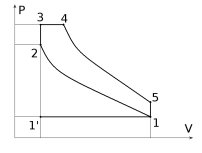
\includegraphics[width=\linewidth]{E6_cycle_diesel}
	\end{center}
\end{minipage}
\hfill
\noindent
\begin{minipage}[c]{.70\linewidth}
	Après la phase d’admission $1' \to 1$ qui amène le mélange au point 1 du
	cycle, celui-ci subit une compression adiabatique supposée réversible jusqu’au
	point 2. Après injection du carburant en 2, la combustion s’effectue d’abord
	de façon isochore de 2 à 3 puis se poursuit de façon isobare de 3 à 4. La
	phase de combustion est suivie d’une détente adiabatique à nouveau prise
	réversible de 4 à 5, puis d’une phase d’échappement isochore $5 \to 1$ puis
	isobare $1 \to 1'$.
\end{minipage}
Au point 1 du cycle, la pression $p_m = \SI{1.0}{bar}$ et la température $T_m =
	\SI{293}{K}$ sont minimales. La pression maximale, aux points 3 et 4, est $p_M =
	\SI{60}{bar}$ et la température maximale, au point 4, vaut $T_M =
	\SI{2073}{K}$. Le rapport volumétrique de compression vaut $\beta = V_M/V_m =
	\num{17}$.
\smallbreak
On suppose que le mélange air-carburant se comporte exactement comme l'air,
c'est-à-dire comme un gaz parfait diatomique de masse molaire $M =
	\SI{29}{g.mol^{-1}}$, et de capacités thermiques respectives $C_P$ et $C_V$.
\QR{%
	Exprimer les températures $T_2$, $T_3$ et $T_5$ en fonction de $p_m$, $p_M$,
	$T_m$, $T_M$ et $\beta$. Calculer les valeurs numériques.
}{%
	solu
}%
\QR{%
	Calculer le transfert thermique massique $q_c$ reçu par l'air au cours de la
	phase de combustion $2 \to 4$.
}{%
	solu
}%
\QR{%
	Calculer le transfert thermique massique $q_f$ échangé avec le milieu
	extérieur entre les points $5$ et $1$.
}{%
	solu
}%
\QR{%
	En déduire le travail massique $w$ échangé au cours d'un cycle.
}{%
	solu
}%
\QR{%
	Définir et calculer le rendement de ce moteur. Commenter la valeur trouvée.
}{%
	solu
}%

\end{document}
